\chapter{Декомпозиция информационной модели АНПА}
\section{Математические выкладки}\label{app:sec:anpa_decompose:calc}

\begin{equation}\label{eq:matrix_a}
    \stackrel{\mbox{Функции}}{%
    A = \begin{pmatrix}
        0 & 0 & 0 & 0 & 0 & 1 & 0 & 0 & 0 & 0 & 1 & 0 & 0 & 0 & 0 & 0 \\
        0 & 0 & 0 & 0 & 0 & 1 & 0 & 0 & 0 & 0 & 0 & 1 & 0 & 0 & 0 & 0 \\
        0 & 0 & 0 & 0 & 0 & 1 & 1 & 0 & 0 & 0 & 0 & 1 & 0 & 0 & 0 & 1 \\
        0 & 0 & 0 & 0 & 0 & 0 & 0 & 1 & 0 & 1 & 0 & 0 & 0 & 0 & 0 & 0 \\
        0 & 1 & 1 & 0 & 0 & 0 & 0 & 0 & 0 & 0 & 1 & 0 & 0 & 1 & 0 & 1 \\
        0 & 0 & 0 & 1 & 1 & 0 & 0 & 0 & 0 & 0 & 0 & 0 & 0 & 0 & 1 & 0 \\
        0 & 0 & 0 & 0 & 0 & 1 & 0 & 0 & 0 & 0 & 0 & 0 & 1 & 0 & 0 & 0 \\
        0 & 0 & 0 & 0 & 0 & 1 & 0 & 0 & 0 & 0 & 0 & 0 & 1 & 0 & 0 & 0 \\
        0 & 0 & 0 & 0 & 0 & 0 & 0 & 0 & 0 & 1 & 0 & 0 & 0 & 0 & 0 & 0 \\
        1 & 1 & 1 & 1 & 1 & 0 & 0 & 0 & 0 & 0 & 0 & 0 & 0 & 1 & 1 & 0 \\
        1 & 1 & 1 & 1 & 1 & 0 & 0 & 0 & 0 & 0 & 0 & 0 & 0 & 1 & 1 & 0 \\
        0 & 0 & 0 & 0 & 0 & 0 & 0 & 0 & 0 & 0 & 0 & 0 & 0 & 1 & 1 & 0 \\
        0 & 0 & 0 & 0 & 0 & 1 & 1 & 1 & 1 & 1 & 1 & 0 & 0 & 0 & 0 & 0 \\
        0 & 0 & 0 & 0 & 0 & 0 & 0 & 0 & 0 & 0 & 1 & 1 & 0 & 0 & 0 & 0 \\
    \end{pmatrix}\rotatebox{270}{\mbox{Объекты}}.
}
\end{equation}


\begin{equation}\label{eq:matrix_b}
    \stackrel{\mbox{Действия}}{%
    B = \begin{pmatrix}
        0 & 0 & 0 & 0 & 0 & 1 \\
        0 & 1 & 0 & 0 & 0 & 0 \\
        0 & 1 & 0 & 0 & 0 & 0 \\
        0 & 0 & 1 & 0 & 0 & 0 \\
        0 & 0 & 1 & 0 & 0 & 0 \\
        0 & 0 & 0 & 1 & 1 & 0 \\
        0 & 0 & 0 & 1 & 1 & 0 \\
        0 & 0 & 0 & 1 & 1 & 0 \\
        0 & 0 & 0 & 1 & 1 & 0 \\
        0 & 0 & 0 & 1 & 1 & 0 \\
        1 & 0 & 0 & 0 & 1 & 0 \\
        1 & 1 & 0 & 0 & 0 & 0 \\
        0 & 1 & 1 & 0 & 0 & 1 \\
        0 & 1 & 0 & 0 & 0 & 1 \\
        0 & 0 & 1 & 0 & 0 & 1 \\
        1 & 0 & 0 & 0 & 1 & 0 \\
    \end{pmatrix}\rotatebox{270}{\mbox{Функции}}.
}
\end{equation}



\begin{equation}\label{eq:matrix_c1}
    C_1 = A \times B = 
    \stackrel{\mbox{Действия}}{%
    \begin{pmatrix}
        1 & 0 & 0 & 1 & 2 & 0 \\
        1 & 1 & 0 & 1 & 1 & 0 \\
        2 & 1 & 0 & 2 & 3 & 0 \\
        0 & 0 & 0 & 2 & 2 & 0 \\
        2 & 3 & 0 & 0 & 2 & 1 \\
        0 & 0 & 3 & 0 & 0 & 1 \\
        0 & 1 & 1 & 1 & 1 & 1 \\
        0 & 1 & 1 & 1 & 1 & 1 \\
        0 & 0 & 0 & 1 & 1 & 0 \\
        0 & 3 & 3 & 0 & 0 & 3 \\
        0 & 3 & 3 & 0 & 0 & 3 \\
        0 & 1 & 1 & 0 & 0 & 2 \\
        1 & 0 & 0 & 5 & 6 & 0 \\
        2 & 1 & 0 & 0 & 1 & 0 \\
    \end{pmatrix}\rotatebox{270}{\mbox{Объекты}}.
}
\end{equation}

\begin{equation}\label{eq:matrix_c2}
    C_2 = \begin{pmatrix}
        \sum_{j=1}^l c_{1\,1j} \\
        \ldots \\
        \sum_{j=1}^l c_{1\,mj} \\
    \end{pmatrix} 
    =
    \begin{pmatrix}
        4 \\
        4 \\
        8 \\
        4 \\
        8 \\
        4 \\
        5 \\
        5 \\
        2 \\
        9 \\
        9 \\
        4 \\
        12 \\
        4 \\
    \end{pmatrix}.
\end{equation}


\begin{equation}\label{eq:matrix_c3}
    C_3 = \left. \frac{C_2}{l} \right|_{l \equiv 6} = 
    \begin{pmatrix}
        0.67 \\
        0.67 \\
        1.33 \\
        0.67 \\
        1.33 \\
        0.67 \\
        0.83 \\
        0.83 \\
        0.33 \\
        1.50 \\
        1.50 \\
        0.67 \\
        2.00 \\
        0.67 \\
    \end{pmatrix}.
\end{equation}


\begin{landscape}
\chapter{Листинги}
\section{Конфигурационный файл параметров сети Modbus}\label{app:sec:modbus_tag}
    \lstinputlisting[
        language=MyXML,
        caption=Конфигурационный файл для описания множества контроллируемых параметров по промышленному протоколу Modbus
            из раздела \ref{sec:modbus_tag}. Файл разметки приведен в листинге \ref{lst:modbus_tags_example_configs}.,
        label=lst:modbus_tags_example]
            {Dissertation/listings/xml/modbus_tags_example.xml}
\end{landscape}

\section{Конфигурация сценария}\label{app:sec:modbus_scenario_example_diagram}
\lstinputlisting[
    language=MyXML,
    caption=Конфигурационный файл примера сценария развития событий (см. рисунок \ref{fig:modbus_scenario_example_diagram}).,
    label=lst:modbus_scenario_example_diagram]
        {Dissertation/listings/xml/modbus_tags_example_scenario.xml}

\begin{landscape}
\section{XML схемы}\label{app:sec:xsd}
    \lstinputlisting[
        language=MyXML,
        caption=Схема разъметки конфигурационного файла из листинга~\ref{lst:modbus_tags_example}.,
        label=lst:modbus_tags_example_configs]
            {Dissertation/listings/xsd/modbus_tags_configs.xsd}
    
    \lstinputlisting[
        language=MyXML,
        caption=Схема разъметки конфигурационного файла из листинга~\ref{lst:modbus_scenario_example_diagram}.,
        label=lst:modbus_tags_scenario_configs]
            {Dissertation/listings/xsd/modbus_tags_scenario_configs.xsd}        
\end{landscape}

\begin{landscape}
    \section{Онтология модели АНПА}\label{app:sec:anpa_owl}
    \lstinputlisting[
        language=MyXML,
        caption=Описание онтологии на языке \texttt{RDF}.,
        label=lst:model_anpa_owl]
            {Dissertation/listings/owl/anpa_2.owl}
\end{landscape}


\chapter{Свидетельство о государственной регистрации программы для ЭВМ}\label{app:sec:registration}
\begin{figure}[hb]\begin{center}
    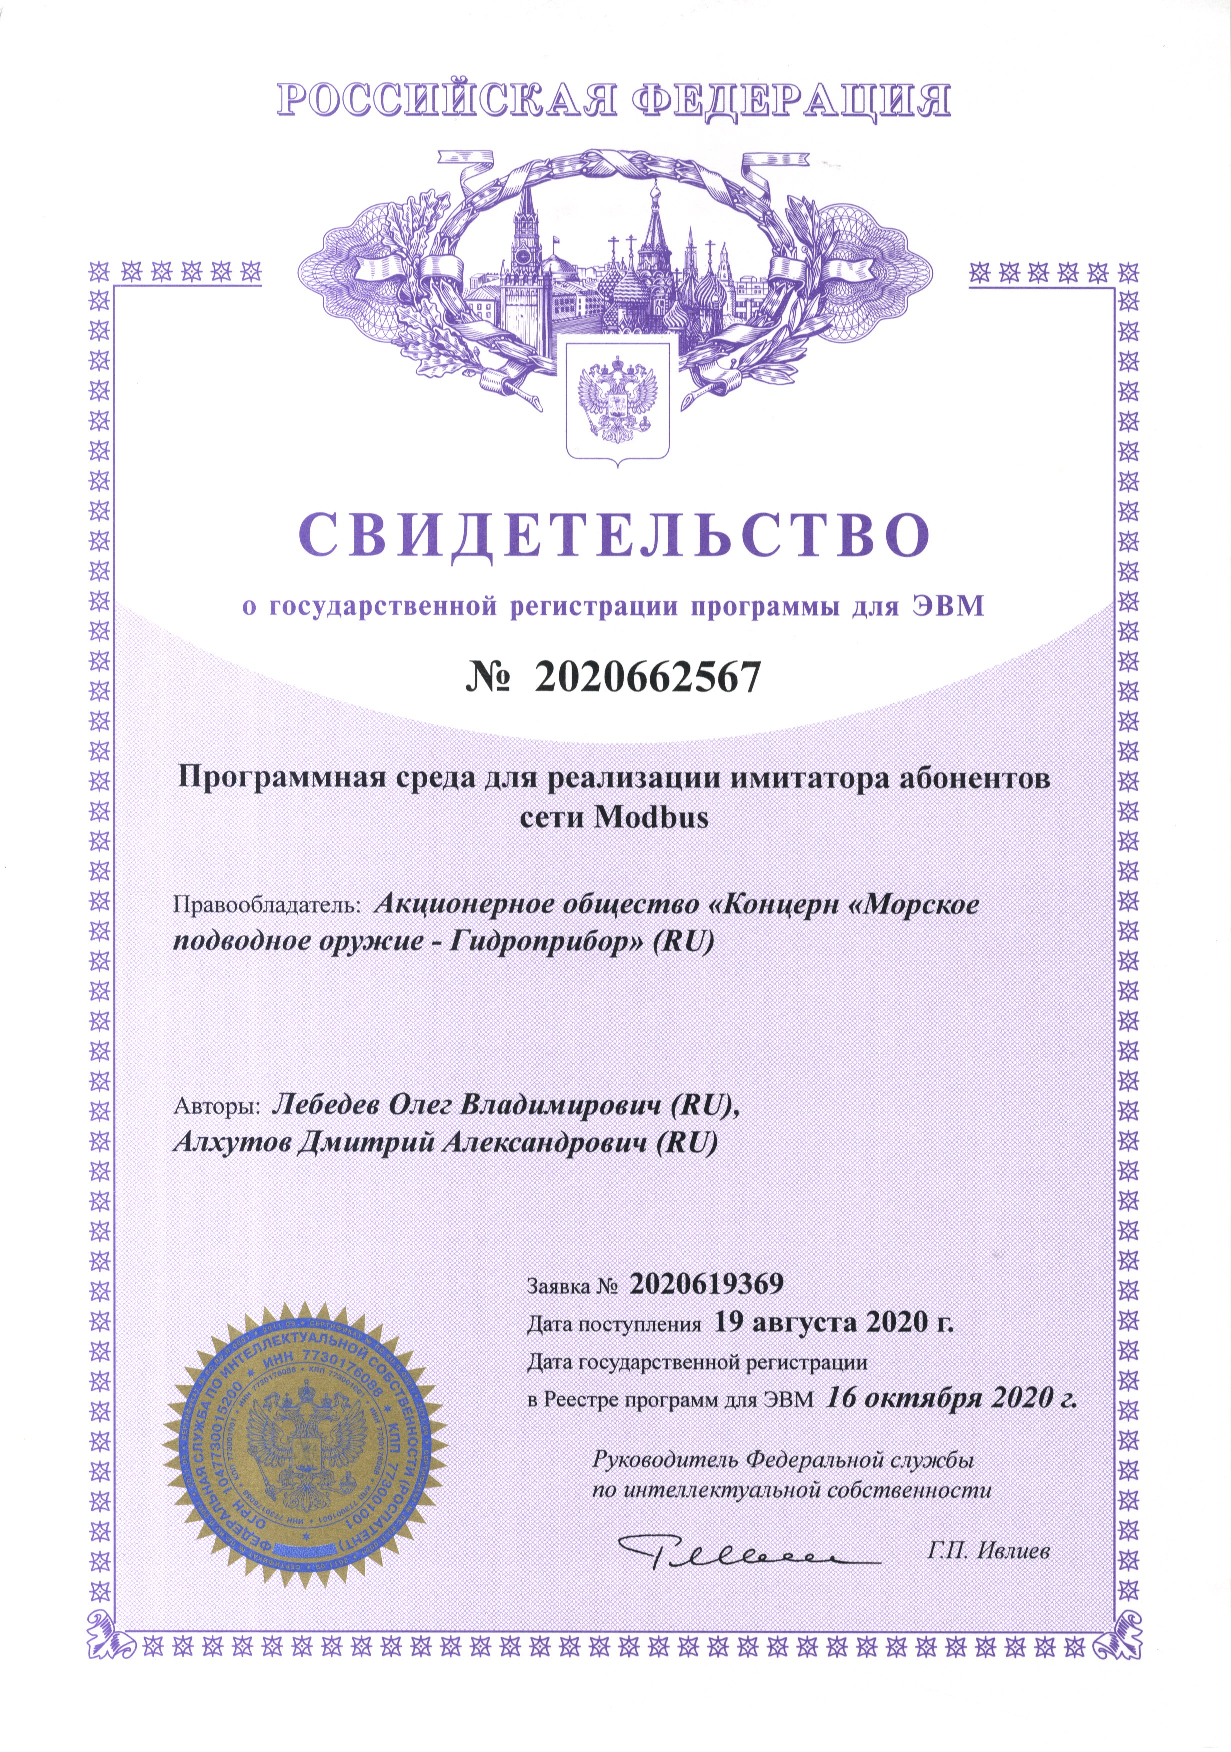
\includegraphics[height=.75\textheight, keepaspectratio]{registration.pdf}
    \caption[Свидетельство о государственной регистрации]
        {Свидетельство о государственной регистрации программы для ЭВМ.}\label{app:fig:registration}
\end{center}\end{figure}


\chapter{Акт о внедрении}\label{app:sec:implementation}
\begin{figure}[hb]\begin{center}
    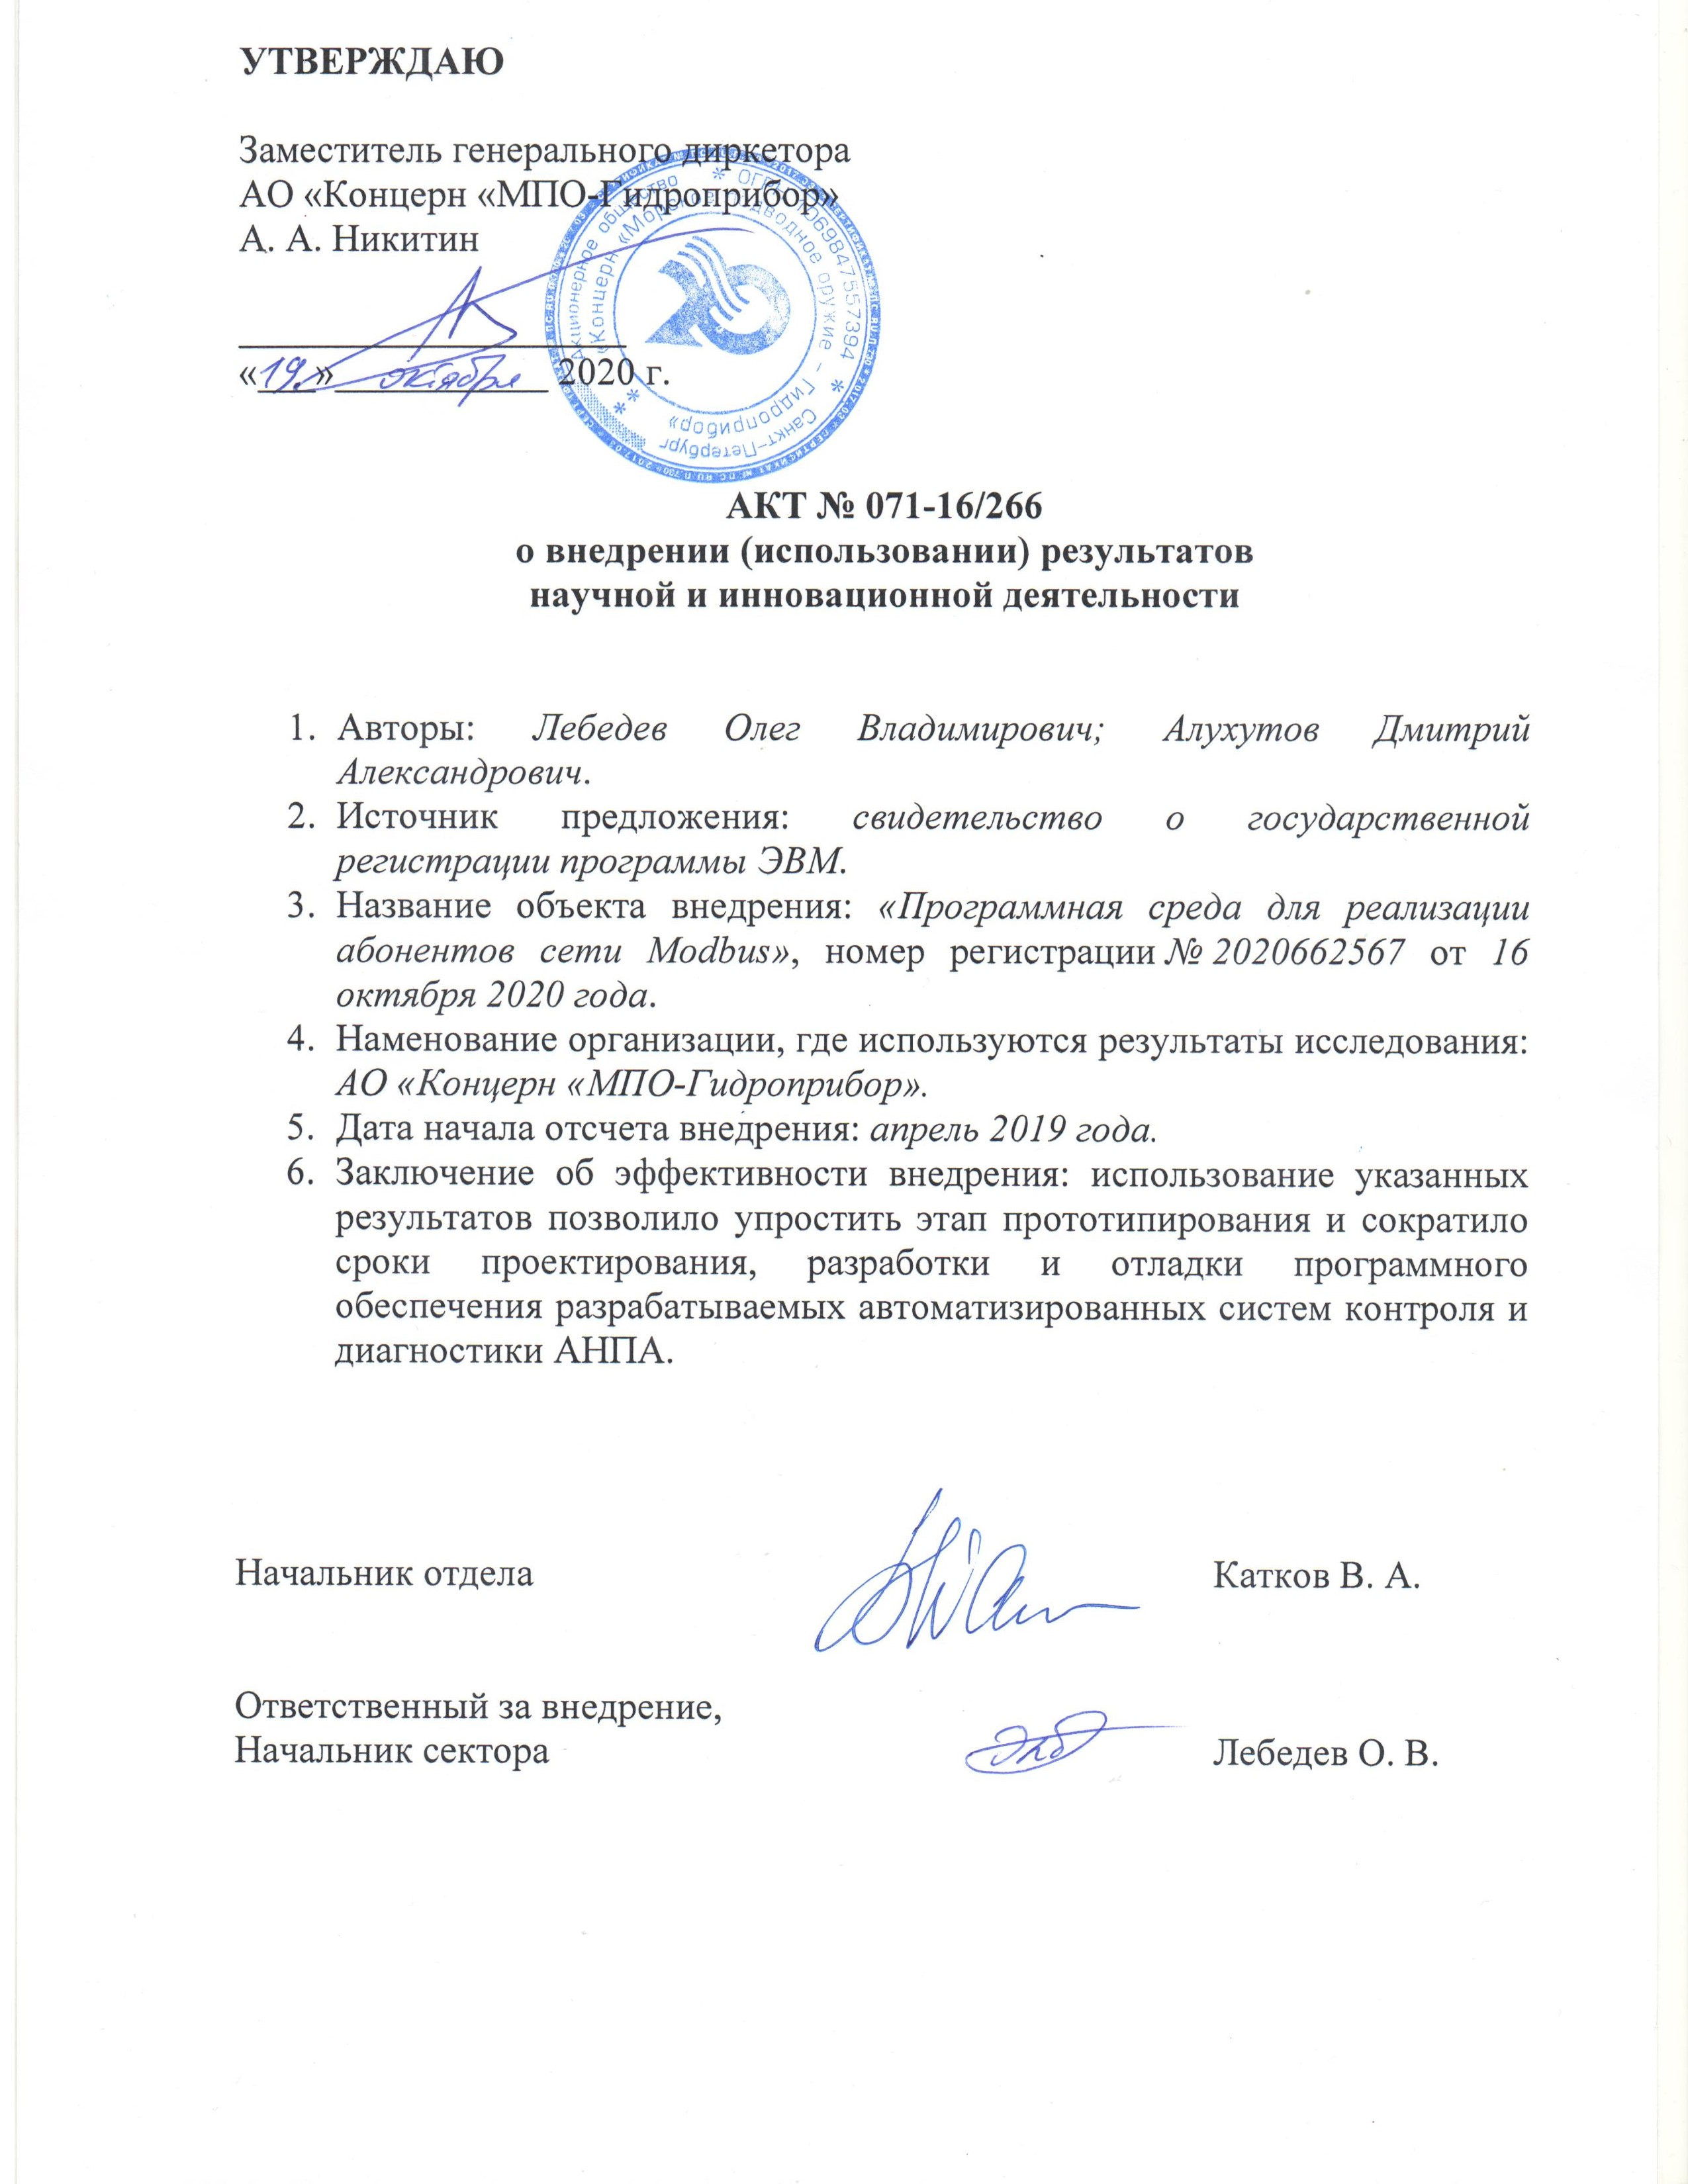
\includegraphics[height=.75\textheight]{implementation}
    \caption[Акт о внедрении]{Акт о внедрении на предприятии \leadingOrganizationTitle.}\label{app:fig:implementation}
\end{center}\end{figure}


\chapter{Дополнительные рисунки}\label{app:sec:figures}
\begin{figure}[hb!]\begin{center}
    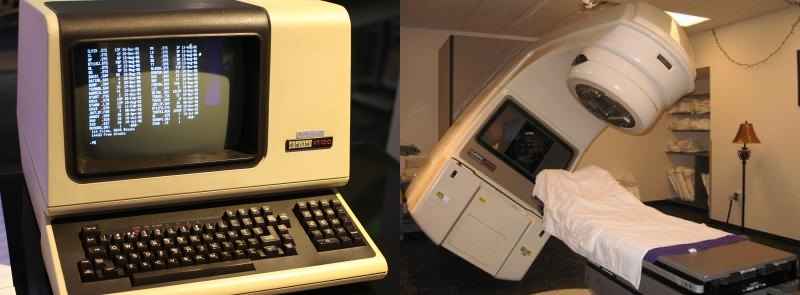
\includegraphics[width=.8\textwidth]{therac25-console}
    \caption[Therac 25]{Therac 25. Консоль оператора показана на рисунке \ref{app:fig:therac25_console}.}
        \label{app:fig:therac25}
    %
    \vspace{10mm}
    %
    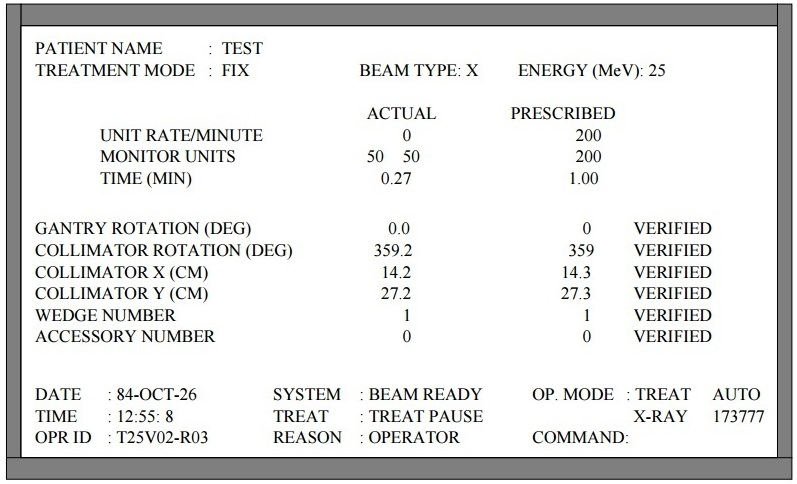
\includegraphics[width=.8\textwidth]{therac25-screenshot}
    \caption[Консоль Therac 25]{Консоль Therac 25.}\label{app:fig:therac25_console}
\end{center}\end{figure}

